\part{Theoretical Background}

\chapter{Theoretical Background}
\label{chap:theoretical_background}

\section{Precision agriculture, water scarcity, and smart irrigation}

Precision agriculture is a data-driven management strategy that adapts agricultural operations to temporal and spatial variability. Instead of treating a field as uniform, it uses measurements, digital tools, and decision-support methods to adjust actions according to local soil, crop, weather, and equipment conditions. In irrigation, this principle is especially important because water demand changes over time and across zones.

Water scarcity is one of the main motivations for smart irrigation. Irrigation based only on fixed schedules can be inefficient because it does not necessarily reflect current soil moisture, crop demand, rainfall, atmospheric demand, or operational constraints. Under-irrigation can cause water stress, poor growth, and yield loss. Over-irrigation can waste water and energy, leach nutrients, increase operating cost, and create salinity or drainage problems. The engineering objective is therefore not simply to irrigate, but to irrigate at the right time, with an appropriate amount of water, and with traceable reasoning.

Smart irrigation uses sensing, communication, data processing, decision support, and sometimes actuators to apply water according to actual need. Kodali and Sarjerao illustrate a low-cost smart-irrigation loop using soil moisture, an ESP8266 controller, MQTT communication, and pump status \cite{kodali2017mqttirrigation}. Balaceanu et al. illustrate the monitoring side of precision agriculture through a Libelium-based platform that collects agricultural and atmospheric variables \cite{balaceanu2019libelium}. These original works show two complementary foundations: irrigation control requires both a physical control loop and reliable environmental information.

\section{Measured variables and irrigation-control components}

Smart irrigation depends on variables that describe soil water availability, atmospheric demand, crop condition, and equipment status. Soil moisture is central because it indicates the water available near the root zone. Soil temperature influences root activity and water uptake. Air temperature, humidity, rainfall, wind, and radiation affect evapotranspiration and the expected drying rate of the soil. Other variables, such as pH, electrical conductivity, pressure, leaf wetness, pump state, and valve state, may be relevant depending on the sensor kit, irrigation infrastructure, and crop.

The vineyard Digital Twin of Bellvert et al. combines field information and Sentinel-2 biophysical variables to support automated irrigation scheduling under regulated deficit irrigation \cite{bellvert2023vineyarddt}. Millan et al. combine soil moisture sensors, climate data, and simulation models in the Irri\_DesK tomato-farm Digital Twin \cite{millan2025tomatodt}. These studies confirm that irrigation support normally requires a coherent set of measurements rather than a single isolated variable.

\begin{table}[H]
\centering
\small
\caption{Common variables and equipment states used in smart irrigation}
\label{tab:background_irrigation_variables}
\begin{tabular}{p{0.24\textwidth}p{0.58\textwidth}}
\hline
\textbf{Category} & \textbf{Examples and irrigation relevance} \\
\hline
Soil variables & Soil moisture, soil temperature, pH, electrical conductivity; indicate root-zone water availability and soil condition. \\
Weather variables & Air temperature, relative humidity, rainfall, wind speed, wind direction, radiation or light; influence evapotranspiration and irrigation timing. \\
Crop indicators & Leaf wetness, crop stage, canopy or biomass indicators when available; help interpret stress and water demand. \\
Hydraulic/equipment state & Pump state, valve state, relay state, line pressure, flow when available; confirms whether irrigation infrastructure can execute or has executed an action. \\
\hline
\end{tabular}
\end{table}

Actuators transform irrigation decisions into physical action. Typical irrigation-control components include pumps, relays, solenoid valves, drip lines, sprinklers, and fertigation injectors. A smart-irrigation system can remain advisory, but when it controls equipment it must also consider safety, feedback, and human supervision. A recommendation should not be treated as equivalent to physical execution unless the actuator state and operational constraints are known.

\section{IoT communication and physical-to-digital connection}

IoT communication is the bridge between physical measurements and digital decision support. A typical irrigation architecture includes sensors, a field node or microcontroller, a gateway, a communication protocol, storage or processing services, a user interface, and sometimes actuators. The field layer observes the physical environment, while the digital layer stores, analyzes, and presents the information.

Several communication technologies are reported in smart-irrigation systems, including Wi-Fi, ZigBee or XBee, LoRa or LoRaWAN, GSM/GPRS, 4G/5G cellular links, Bluetooth, and wired connections. The choice depends on range, energy consumption, bandwidth, cost, deployment environment, and reliability. MQTT is frequently used in IoT because it provides a lightweight publish/subscribe model. Devices publish messages, a broker routes them, and services subscribe to the information they need. At this conceptual level, exact topic names and payload structures are not discussed; those details belong to implementation chapters.

The physical-to-digital connection is not only a communication problem. It also requires calibration, timestamping, missing-data handling, unit normalization, and device identification. If these elements are weak, the digital representation can diverge from the physical situation. Therefore, sensing and communication must be treated as part of the Digital Twin foundation rather than as separate accessories.

\section{Digital Twin, machine learning, and human-in-the-loop decision support}

A Digital Twin is a synchronized virtual representation of a physical system. It is more than a static model or a dashboard because it receives data from the physical system, updates its state, and supports reasoning about possible actions. In irrigation, a Digital Twin can maintain the state of a zone, integrate sensor and weather data, simulate moisture evolution, support recommendations, and connect decisions to control workflows.

\begin{table}[H]
\centering
\small
\caption{Distinction between digital representations}
\label{tab:digital_model_shadow_twin}
\begin{tabular}{p{0.24\textwidth}p{0.58\textwidth}}
\hline
\textbf{Representation} & \textbf{Data-flow meaning} \\
\hline
Digital Model & Offline or manually updated representation; changes in the physical system do not automatically update the digital model. \\
Digital Shadow & One-way data flow from the physical system to the digital representation; the virtual state follows measurements but does not necessarily influence the physical system. \\
Digital Twin & Bidirectional cyber-physical connection where measured data update the virtual state and digital reasoning can support recommendations, scheduling, or supervised control. \\
\hline
\end{tabular}
\end{table}

Machine learning can support irrigation by learning relationships between measurements and irrigation outcomes. Models may classify whether irrigation is needed, estimate soil moisture evolution, forecast water demand, or suggest an irrigation time. Tancredi et al. investigate a Digital Twin enhanced with machine-learning algorithms for irrigation management using sensor data \cite{tancredi2025irrigationdt}. Ed-Daoudi et al. also position predictive irrigation as a combination of IoT sensing, machine learning, and adaptive scheduling \cite{eddaoudi2024predictiveirrigation}. Figure~\ref{fig:tancredi-ml-dt-irrigation} reproduces the ML-enhanced Digital Twin framework used as a conceptual reference.

\begin{figure}[H]
    \centering
    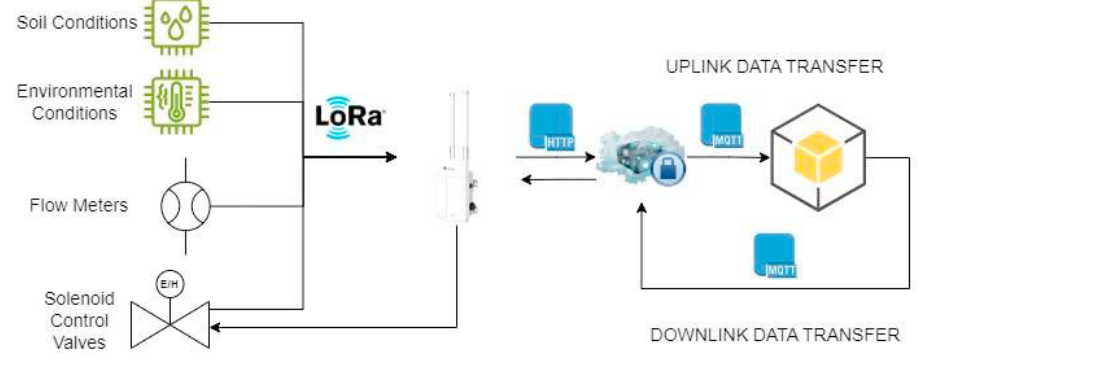
\includegraphics[width=0.85\textwidth]{figures/research_papers/tancredi_ml_dt_irrigation.png}
    \caption{Machine-learning-enhanced Digital Twin framework for irrigation management. Reproduced unchanged from Tancredi et al.~\cite{tancredi2025irrigationdt}.}
    \label{fig:tancredi-ml-dt-irrigation}
\end{figure}

Bellvert et al. describe a Digital Twin and IoT-based application for vineyard irrigation scheduling \cite{bellvert2023vineyarddt}, while Millan et al. evaluate a Digital Twin workflow for water-efficient tomato-farm management \cite{millan2025tomatodt}. Figure~\ref{fig:bellvert-vineyard-dt-scheduling} illustrates scheduling parameters from Bellvert et al.

\begin{figure}[H]
    \centering
    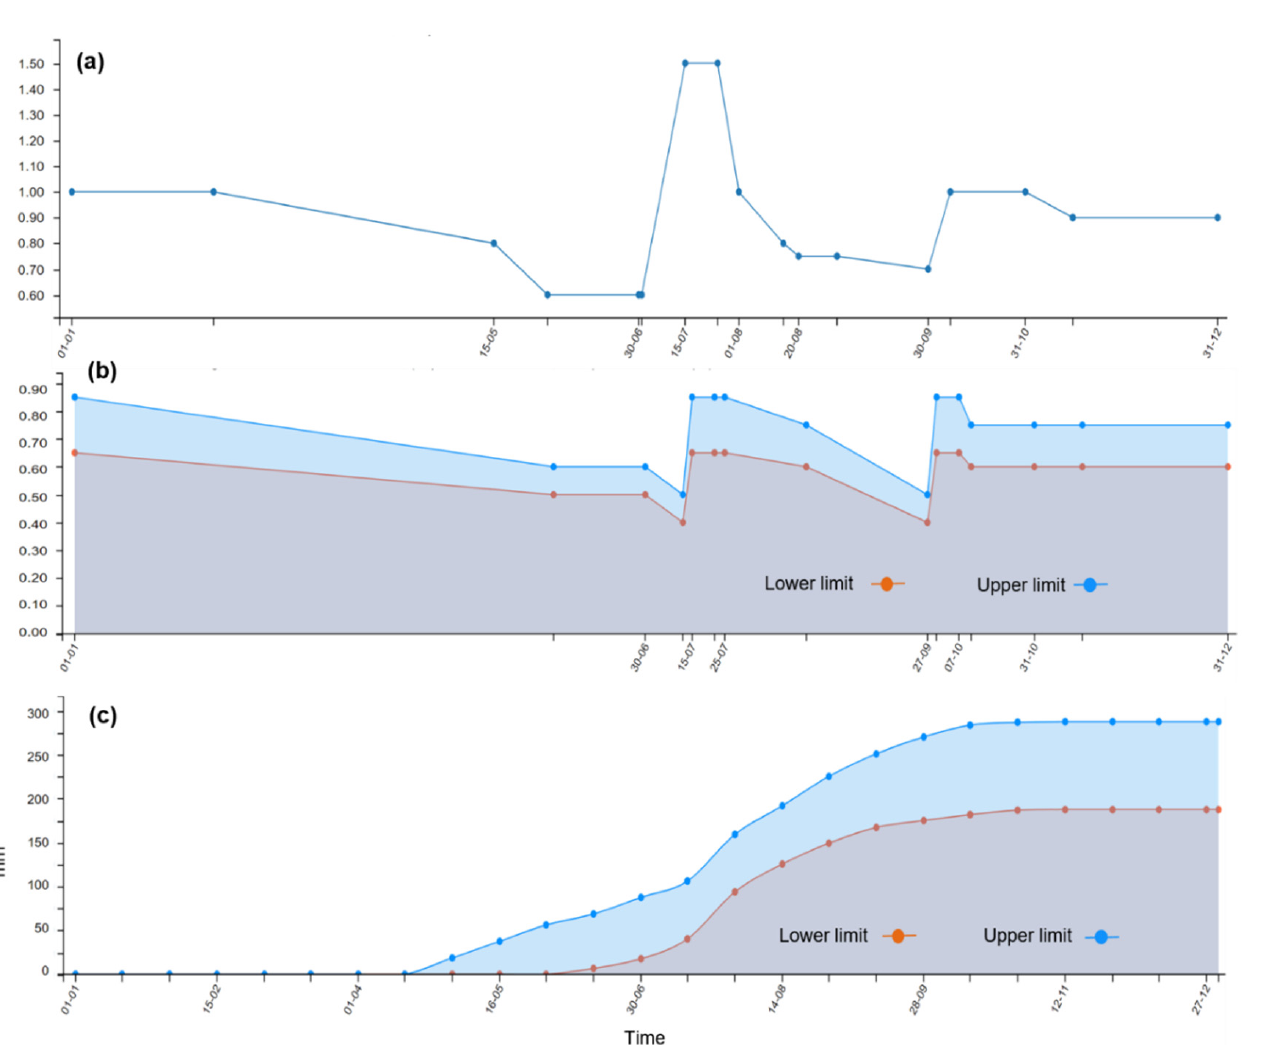
\includegraphics[width=0.9\textwidth]{figures/research_papers/bellvert_vineyard_dt.png}
    \caption{Seasonal-plan parameters used for automated vineyard irrigation scheduling. Reproduced from Bellvert et al.~\cite{bellvert2023vineyarddt}.}
    \label{fig:bellvert-vineyard-dt-scheduling}
\end{figure}

Digital Twin maturity can be understood as a progression from monitoring to prediction, simulation, recommendation, scheduling, and control. Monitoring observes current conditions. Prediction estimates needs or future states. Simulation compares possible actions before they are executed. Recommendation converts analysis into user-readable advice. Scheduling transforms accepted decisions into planned events. Control sends commands to physical equipment.

Human-in-the-loop decision support is important because irrigation has physical and agronomic consequences. A false positive recommendation can waste water or damage the crop through over-irrigation, while a false negative recommendation can expose plants to stress. Human validation also improves trust: the user can inspect sensor values, predictions, scenario results, and reasons before allowing physical execution.

\section{Summary}

This chapter strengthened the conceptual background of the thesis. Precision agriculture motivates data-driven irrigation under water scarcity. Smart irrigation combines measured variables, communication, processing, decision support, and actuators. Digital Twins add synchronized virtual state, simulation, recommendation, scheduling, and possible supervised control. Key challenges remain: sensor calibration, wireless reliability, missing data, interoperability, cybersecurity, agronomic calibration, field validation, usability, and user trust. The next chapter analyzes related original research systems and compares how they address these functions.
